\documentclass{beamer}
\usepackage[utf8]{inputenc}
\usepackage{beamerthemeshadow}

\usetheme{Berlin}
\title[Temperature Sensing]{Miniproject 3 \\ Temperature Sensing}
\author{Frederik Mogensen,\\
    Allan Stisen,\\
    Lasse Højgaard }
\date{\today}
\begin{document}
 \AtBeginSection[]
{
  \begin{frame}
    \tableofcontents[currentsection]
  \end{frame}
}
\begin{frame}
\titlepage
\end{frame}

\section{Project Description}


\begin{frame}
\frametitle{Description}

\begin{itemize}
	\item make a  sensor network which can measure the temperature periodically
	\item Sensor mote transmit results to sink
	\item Sensor shows the results by either:
	\begin{itemize}
		\item a blue ($\leq 15^{\circ} C $) led
		\item or a red $>15^{\circ} C$ led 
	\end{itemize}
	\item Sink sends ACK to sensor mote if receives package
	\item Sensor mote goes to sleep if receives ACK or try to retransmit $N$ times.
\end{itemize}
\end{frame}

\begin{frame}
\frametitle{Extensions of project}
\begin{description}
\item[Multiple motes] If there are multiple sensing motes, they send their sensing data to the sink.
\item[Plotting] Plot temperature vs. time (offline /online)
\item[Temperature average] The sink averages the temperature from the sensors.
\item[Temperature average sensor] The sensor motes averages $n$ temperatures before sending to the sink to improve energy efficiency of the application.
\item[Temperature average improved] Motes averages temperature sends number of recorded temperatures which indicates what weight the sink should use to make a correct average.

\end{description}
\end{frame}

\section{Project implementation}
\begin{frame}
\frametitle{Project overview}
\begin{figure}[htbp]
   \centering
   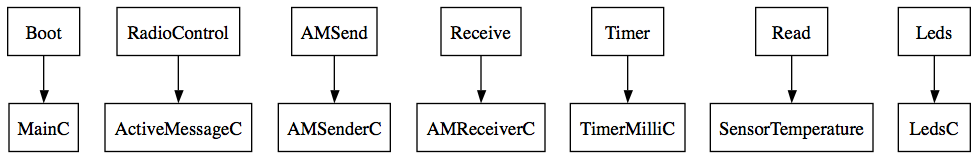
\includegraphics[width=11cm]{SWgraph.png} 
\end{figure}

\end{frame}

\begin{frame}
\frametitle{Temperature measuring}
The conversion given a digital readout ($SO_{T}$) to a temperature value is given at the following formula:
\begin{align*}
	T &= d_{1} + d_{2} \cdot SO_{T}
\end{align*}
where the coefficients is the following
\begin{table}[ht]
\centering
\begin{tabular}{ | l | c | r | }
	\hline
	VDD & $d_{1} \ ^{\circ}  C$ & $d_{1} \ ^{\circ}  F$ \\
	\hline \hline
	5V & -40.1 & -40.2 \\
	\hline
	4V & -39.8 & -39.6 \\
	\hline
	3.5V & -39.7 & -39.5 \\
	\hline
	3V & -39.6 & -39.3 \\
	\hline
	2.5V & -39.4 & -38.9 \\
	\hline
\end{tabular}
\begin{tabular}{ | l | c | r | }
	\hline
	$SO_{T}$ & $d_{2}  \ ^{\circ}C$ & $d_{2} \ ^{\circ} F$ \\
	\hline \hline
	14 bit & 0.01 & 0.018 \\
	\hline
	12 bit & 0.04 & 0.072\\
	\hline
\end{tabular}
\caption{Temperature conversion coefficients}
\label{table:temperature}
\end{table}

\end{frame}

\begin{frame}
\frametitle{Package transfer and receive}

\end{frame}


\section{Project results}

\begin{frame}
\frametitle{Project results}
 
\end{frame}

\end{document}
